% !TEX root = ../main.tex
% Visualisierung

% Kapitel \ref{chap:daten} gibt einen "Uberblick "uber gr"o"se und Struktur der genutzten Datens"atze um nachvollziehen zu k"onnen welche Daten visualisiert werden.
In diesem Kapitel wird auf die gewählte Darstellung von Kategorien eingegangen und welche Interaktionsmöglichkeiten die Visualisierung bietet.
Darüber hinaus wird verdeutlicht, welche nicht sichtbaren Veränderungen während der Laufzeit des Programms an den Daten vorgenommen werden.
Die in Kapitel \ref{chap:daten} eingeführten Datensätze werden in diesem Kapitel vertiefend erklärt. Auf dieser Basis wird gezeigt, wie sie zur visuellen Repräsentation verknüpft werden.
Im Gegensatz zur Visualisierung des Projekts \emph{Visual Text Analytics} stehen die Verbindungen zwischen den Kategorien im Mittelpunkt der angestrebten Darstellung.
Der Ansatz, möglichst viele Artikel und ihre Ähnlichkeiten abzubilden, wurde verworfen, da über den direkten Zugang zu den Artikeln die Menge an Vergleichen zwischen den Artikeln so groß würde, dass eine vereinfachte, überschaubare Darstellung der Informationen schwerlich gelingen könnte.
Stattdessen sollen die Kategorien einen abstrakteren Zugang zu den Artikeln schaffen, die Übersichtlichkeit stärken und die Auswahl an Artikeln auf ein Themengebiet beschränken.

% notizen  was muss rein
Der Grundgedanke der Arbeit liegt in der Annahme, die Kategorienstruktur als Hierarchie von Abstraktionsebenen zu interpretieren.
Dabei sollen Kategorien, die in der Hierarchie höher sind, also näher am Stammverzeichnis liegen, Themengebiete prägnant beschreiben. Die Kategorien, welche in der Hierarchie weiter unten stehen, sollen hingegen eine ausführlichere Beschreibung des Gegenstands bieten.
Diese Annahme wird durch die vermeintliche Ordnung unterstützt, die aus den Kategorien selbst hervorgeht.
Wesentlich für die Hierarchie ist die Bestimmung eines Stammverzeichnisses der Kategorien.
Wichtige Eigenschaften für ein Stammverzeichnis sind die grundlegende Betrachtung von Artikelseiten, als auch eine Betrachtung der Abstraktionsebene, welche maximal viele weit gefasste Themengebiete als Unterkategorie eingetragen hat.
Die Wikipedia markiert die Kategorie \emph{Contents} \footnote{\url{https://en.wikipedia.org/wiki/Category:Contents}} als Stammverzeichnis aller Kategorieseiten. Diese Seite ist gleichwohl ungeeignet für die Nutzung als Stammverzeichnis, da in ihr auch Kategorien aus Namensräumen außerhalb der Artikelseiten eingetragen sind.
In dieser Arbeit wird die Kategorie \emph{Main Topic Classifications} \footnote{\url{https://en.wikipedia.org/wiki/Category:Main_topic_classifications}} als Stammverzeichnis gewählt.
In ihren Unterkategorien sind hauptsächlich Artikelseiten eingetragen und die Unterkategorien, welche die Wikipedia enthält, unterteilen sie in 22 Themengebiete.
Folglich erfüllt sie alle zuvor verlangten Eigenschaften.
Die zweite Eigenschaft, neben dem Stammverzeichnis für eine hierarchisches Modell, ist die Ordnung der Kategorien untereinander.
Auf der Seite \emph{Main Topic Classifications} wird darauf hingewiesen, das die Kategorienstruktur nicht als strikt hierarchisch verstanden werden soll. Daraus lässt sich schließen, dass Kategorien in einem Graph miteinander verbunden sind.
Die genauere Betrachtung der Verbindungen der Kategorien veranschaulicht ihren Charakter.
Besteht eine Verbindung zwischen zwei Kategorien, werden diese jeweils in der anderen eingetragen.
Diese Verbindung geschieht nicht gleichberechtigt, sondern besitzt eine Gewichtung. Denn die eingetragene Kategorie wird entweder als Unterkategorie oder als Oberkategorie eingetragen.
Daraus lässt sich folgern, dass der Graph, bestehend aus Verbindungen zwischen Kategorien, ein gerichteter Graph ist.
In einem weiteren Schritt wird der gerichtete Graph traversiert und die Kategorien werden in Form eines Baums konstruiert. Dabei sollen die Kanten verworfen werden, welche die Kategorien einer Ebene mit einer höheren Ebene verbinden.
Das Kapitel \nameref{chap:Implementierung} schildert den verwendeten Algorithmus, welcher aus dem gerichteten Graphen ein Baumdiagramm konstruiert.
Dieser Kategorienbaum, in dem die Hierarchie der Kategorien modelliert wird, ermöglicht eine \emph{Top-Down} -Struktur \footnote{\url{https://de.wikipedia.org/wiki/Top-down_und_Bottom-up}} von Kategorien hin zu einzelnen Artikeln.
Der \emph{Top-Down}-Ansatz entspricht dem Kerngedanken der Exploration der Datensätze. Im Folgendem wird die visuelle Umsetzung dieses Ansatzes erläutert.

% \begin{itemize}
%     \item Layoutalgorithmus f"ur Knoten (Eades Free Tree)
%     \item Anordnung der Beschriftungen der Kategorien
% \end{itemize}
\begin{figure}
    \centering
    \begin{tikzpicture}
    \node[draw=red, very thick] (fig) at (3,3) {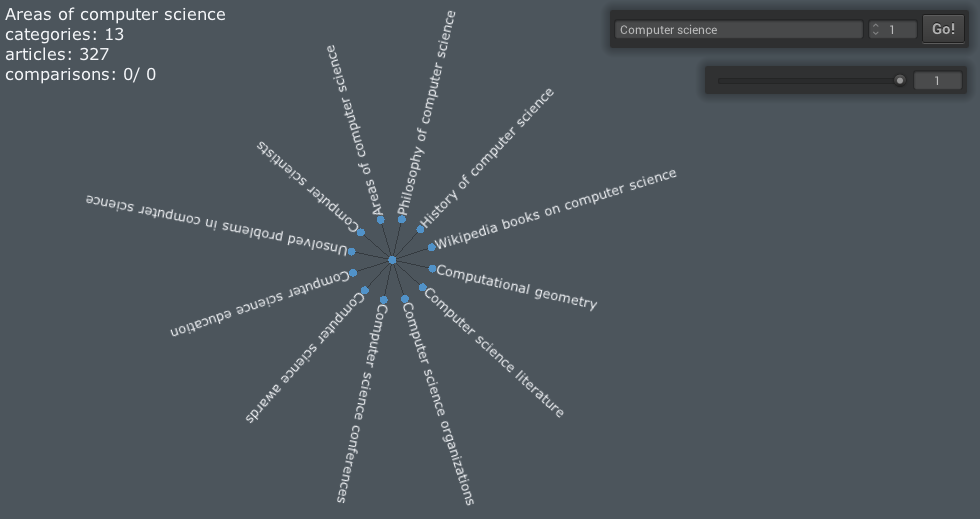
\includegraphics[width=\textwidth]{images/small-start-cs-lvl1.png}};
    \node[red, below] at (fig.south) {(a)};
    
    \node (one) at(-3.3,6.6) [rectangle, draw=red, very thick, inner sep=0pt, minimum width=3.9cm, minimum height=1.5cm]{};
    \node[red, below] at (one.south) {(b)};
    
    \node (two) at(8,6.9) [rectangle, draw=red, very thick, inner sep=0pt, minimum width=6.2cm, minimum height=.75cm]{};
    \node[red, above] at (4.5, 6.6){(c)};
    \node (three) at(8.8,6) [rectangle, draw=red, very thick, inner sep=0pt, minimum width=4.6cm, minimum height=.6cm]{};
    \node[red, below] at (three.south) {(d)};
    \end{tikzpicture}
    \caption{Darstellung der Kategorie \emph{Computer science} im Zentrum des radialen Graphen.
    Es sind die Unterkategorien mit einer Tiefe von eins, mit der Stammkategorie verbunden und sichtbar.\\ (a) Hauptfenster, (b) zusammenfassende Statistik über vorhandene Daten, (c) Suchleiste, (d) Regler zur Änderung des Schwellwerts}
    \label{fig:small-start}
\end{figure}

\section{Layout}
Es gibt verschiedene Möglichkeiten Bäume anzuordnen, bekannte Methoden sind die horizontale oder vertikale Ausrichtung des Baumes.
In dieser Arbeit wurde sich dazu entschlossen den Baum radial anzuordnen, da auf diese Weise gewährleistet wird, das der verfügbare Platz optimal genutzt wird. \footnote{\cite[Kapitel 5, p.~123]{lima2014book}}

% Einführend zu diesem Kapitel wird auf die Taxonomie von Kreisdarstellungen nach \cite[p.~57]{lima2017circle} eingegangen.
% Lima beschreibt zwölf wesentliche Merkmale von Kreisen, dabei gehen wir nur auf Merkmale ein die eine zentrale Rolle in der Visualisierung einnehmen.

Im Folgendem werden die Merkmale für Kresidarstellungen aus der Taxonomie von Kreisen nach \cite[p.~57]{lima2017circle} genutzt.
Kategorien werden als Knoten in Form von blau gefärbten Kreisen dargestellt.
Verbindungen zwischen Kategorien werden als Kanten in Form von schwarze Linien zwischen zwei Knoten dargestellt.
Nachstehend wird der Begriff der Kategorie stellvertretend für die visuelle Form eines Knoten genutzt.
Die im Zentrum des Baumes liegende Kategorie repräsentiert die Stammkategorie und wird auch Wurzel genannt, alle dargestellten Knoten sind durch Kanten mit Ihr verbunden.
Kategorien die keine Unterkategorien besitzen werden Blattkategorien gennant.
Die Unterkategorien der Wurzelkategorie werden auf konzentrischen Ringen um die Wurzelkategorie angeordnet, dabei haben alle Unterkategorien die auf einem Ring liegen die gleiche Distanz zur Wurzelkategorie.
Die Distanz zwischen zwei Kategorien wird festgelegt durch die Anzahl an Kanten, die auf dem kürzestem Pfad zwischen den beiden Kategorien liegen, sie wird auch als Tiefe der Kategorie umschrieben.
Kozentrische Ringe haben auch eine Tiefe zur Wurzelkategorie.
Die Anzahl an konzentrischen Ringen wird bestimmt durch die tiefste dargestellte Kategorie.
Die Anzahl an Sektoren wird bestimmt durch die Anzahl an von Unterkategorien der Tiefe eins, die Breite eines Sektors wird bestimmt durch die Anzahl an Blattkategorien die Nachfolger einer Unterkategorie der Tiefe eins sind.



Der Begriff Tiefe wird genutzt, da ausgehend von der Wurzelkategorie die 
Die Wurzelkategorie ist auch immer die initiale Kategorie nach der gesucht wurde.
Allen voran ist die konzentrische Ausrichtung der 



% Notizen ingnorieren =================
% Ebene --> ringe!!
% Warum ein radiales Layout? warum konzentrisch, Welche Eigenschafte  sind gefragt und welche werden erfüllt.
% Ausnutzen des gesamte Raums?
% Konkrete Struktur des Kategorienbaums ist nicht klar.

% Wie funktioniert der Algorithmus von Eades?
% fokus aug Knoten statt Kanten.
% Strategie der beschriftung der Knoten.
%  ====================================








\begin{figure}
    \centering
    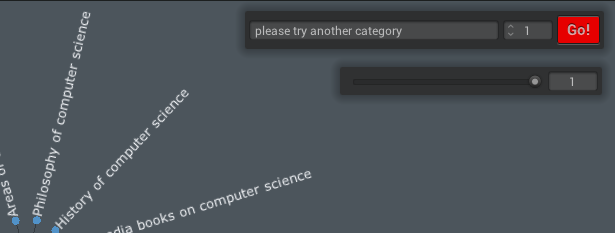
\includegraphics[scale=.5]{images/small-start-wrong-cat-1.png}
    \caption{Ein Nutzer hat bereits nach einer Kategorie gesucht, welche nicht in der Datenbank gefunden wurde. Der Nutzer wird durch die Graphische Benutzeroberfläche aufgefordert die Suche zu wiederholen.}
    \label{fig:wrong-cat}
\end{figure}

% \begin{itemize}
%     \item Expansion von Kategorien
%     \item Schwellwert f"ur "Ahnlichkeitswerte
%     \item Navigation
% \end{itemize}
\section{Interaktion}
Die Interaktionen mit der Visualisierung lassen sich in zwei Gruppen einteilen, ein Nutzer kann entweder mit der graphischen Benutzeroberfläche interagieren, in Abbildung \ref{fig:small-start} mit (c) und (d) markiert oder ein Nutzer interagiert direkt mit den Inhalten im Hauptfenster in der Abbildung gekennzeichnet mit (a).
Nachfolgend werde sollen die Möglichkeiten erläutert werden.

\paragraph{Graphische Benutzeroberfläche}
Das Element (c) aus der Abbildung \ref{fig:small-start} ist Teil der graphischen Benutzeroberfläche und stellt eine Suchleiste für alle Kategorien der Wikipedia da.
Die Suchleiste ist dabei aus drei Elementen aufgebaut, dem Suchformular, dem Eingabefeld für die Tiefe und eine Schaltfläche.
In der Suchleiste kann der Name einer möglichen Kategorie eingegeben werden, drück ein Nutzer nach der Eingabe einer Kategorie die Schaltfläche "`Go!"' wird eine Suchanfrage mit der eingegebenen Kategorie an die Datenbank weitergeleitet.
Existiert keine Kategorie unter dem eingegebenem Namen, wird die Schaltfläche "'Go!"` rot gefärbt und der Nutzer aufgefordert eine andere Kategorie einzugeben.
Existiert die Kategorie stattdessen in der Datenbank wird ein Kategorienbaum mit der Anzahl an Ebenen, welche im Eingabefeld für die Tiefe eingetragen ist gezeichnet und mit der gesuchten Kategorie im Zentrum dargestellt.
Das Eingabefeld für die Tiefe des Kategorienbaums kann durch Eingabe des Nutzers verändert werden, dies ist über die Tastatur oder über die Pfeile im Eingabefeld möglich.
Die Zahl legt die minimale Tiefe des Kategorienbaums fest, dies bedeutet, dass den Blattkategorien solange Unterkategorien hinzugefügt werden, bis sie die eingegebene Tiefe erreichen.
Daraufhin ist die Distanz zwischen  Blattkategorien und der Wurzelkategorie mindestens so groß wie die eingegebene Tiefe, die Expansion der Blattkategorien wird durch drücken der Schaltfläche "`Go!"' bestätigt.
Dabei bleiben bereits gezeichnete Kategorien die Tiefer sind als die Eingabetiefe unverändert in der Visualisierung.

Das andere Elemente der Graphischen Benutzeroberfläche ist der Regler zur Veränderung des Schwellwertes der Ähnlichkeitswerte, in Abbildung \ref{fig:small-start} gekennzeichnet mit (d).
Das Element besteht dabei aus zwei Feldern, einem Schieberegler und einem Zahlenfeld um den eingestellten Wert ablesen zu können.
Der Schieberegler ändert an erster Stellen keine sichtbaren Schwellwert sondern gibt eine Grenze an für den Datensatz von Artikelähnlichkeiten an.
Der Schieberegler stellt dabei die Mindestgröße für Ähnlichkeitswerte ein, die der Ähnlichkeitswert zwischen zwei Artikel überschreiten muss.
Artikelpaare mit einem Ähnlichkeitswert die niedriger sind als der Schwellwert werden nicht in Betracht gezogen.
% Die Veränderung des Schiebereglers ändert neben dem Schwellwert auch die Farbe Knoten von blau nach gelb.
Der visuelle Effekt des Schieberegler ist die Färbung von Knoten von blau nach gelb.
Kategorien werden gelb gefärbt wenn Artikel darin eingetragen sind, die eine Ähnlichkeit zu einem Artikel aus einer dargestellten Kategorie besitzten, die höher oder gleich dem Schwellwert ist.
Der Schieberegler zeigt damit die Kategorien an, die Artikelpärchen eingetragen haben mit einer Ähnlichkeit über oder gleich dem Schwellwert.
Diese Form der Filterung der dünn besetzten Ähnlichkeitsmatrix, nennen wir horizontale Siebung, abbildung  soll dies Verdeutlichen.
\begin{figure}
    \centering
    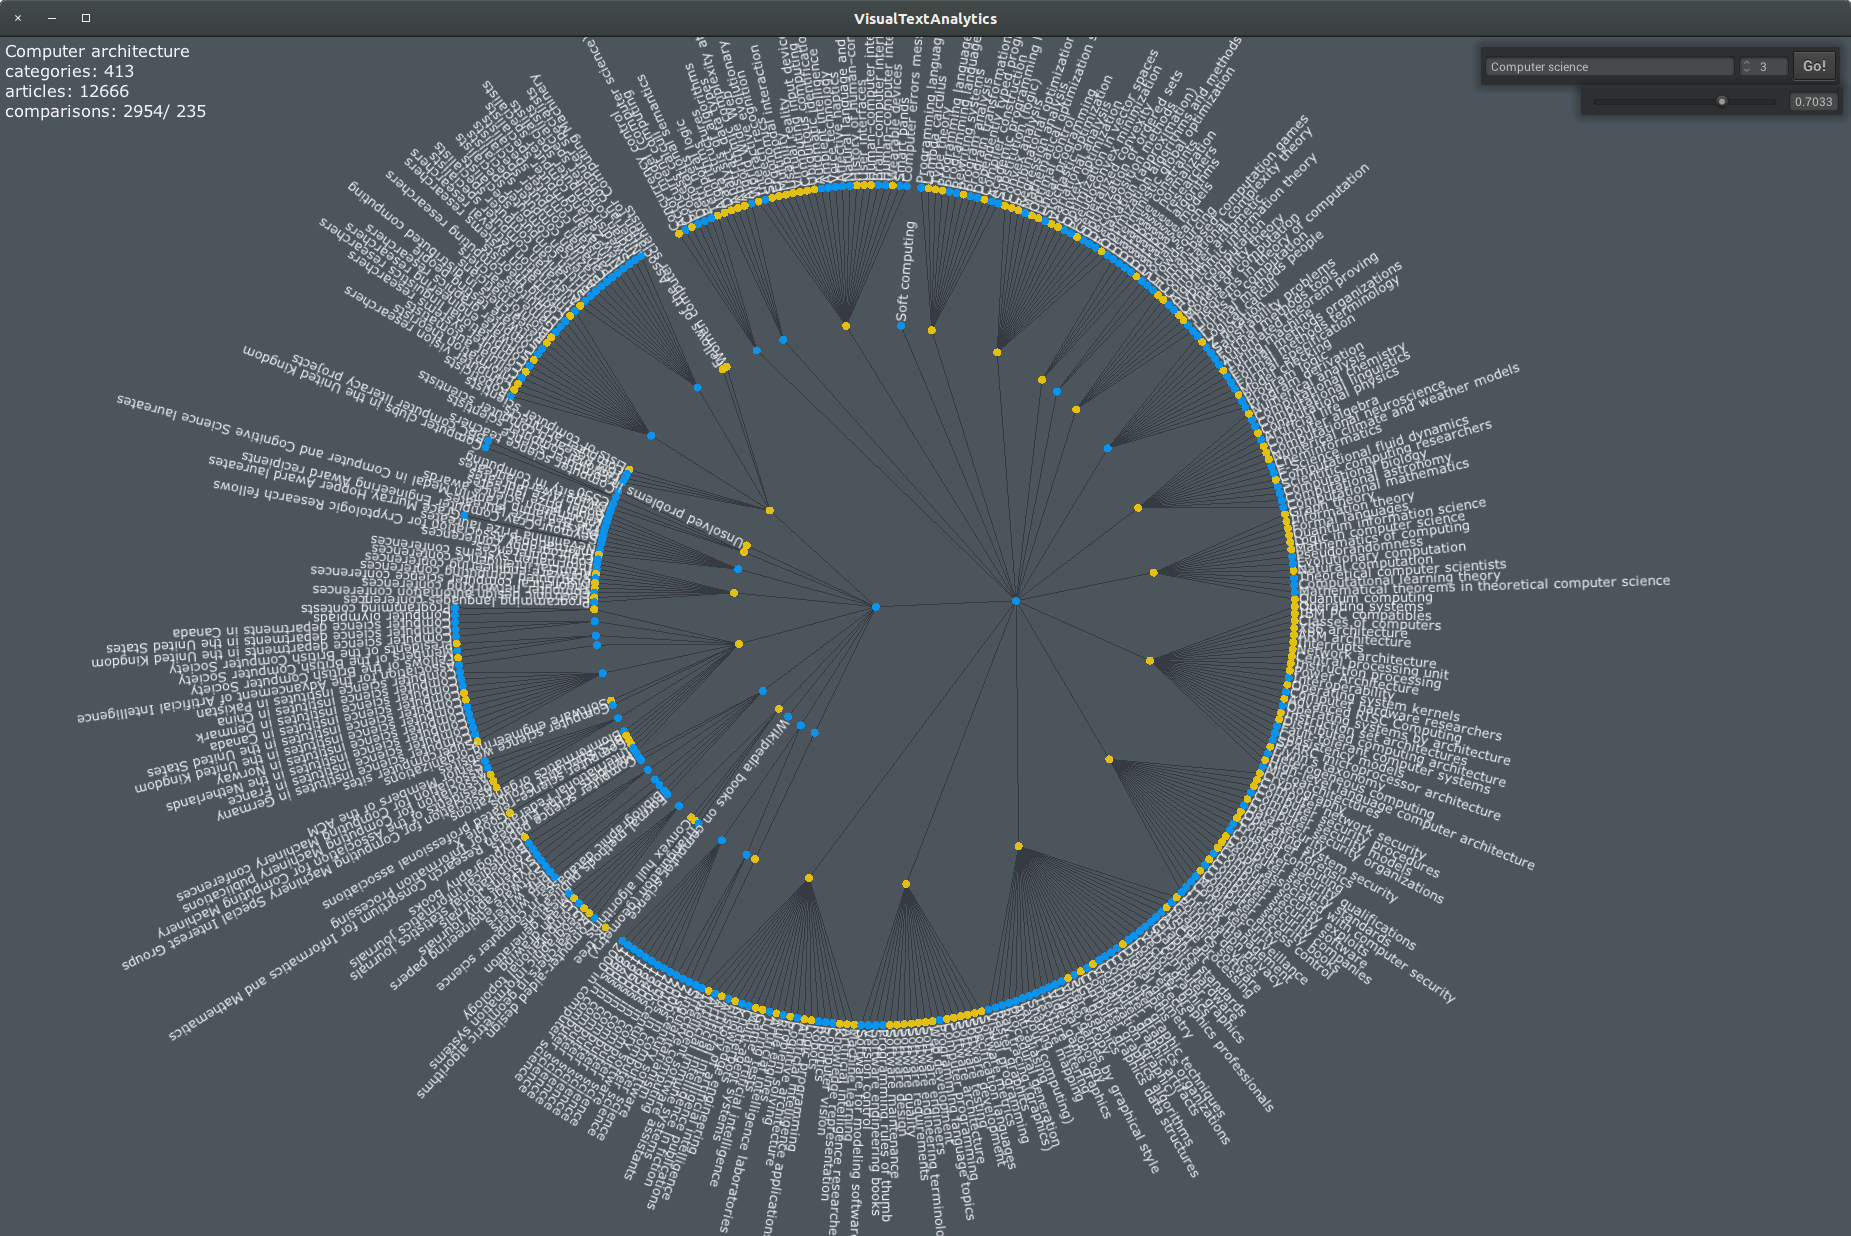
\includegraphics[width=\textwidth]{images/threshold-7033-lvl3}
    \caption{Färbung von Kategorien über dem Schwellwert, Eingabe des Schwellwertes}
    \label{fig:threshold-cat}
\end{figure}

\begin{figure}
    \begin{tikzpicture}
    \end{tikzpicture}
    \caption{Darstellung der filterung der Ähnlichkeitsmatrix die durch den Schwellwert entstehen}
    \label{fig:simM-threshold-cat}
\end{figure}

\paragraph{Hauptfenster}
Mit dem Hauptfenster wird der Bereich gemeint der in Abbildung \ref{fig:small-start} mit (a) markiert ist, ausschließlich der Elemente (c) und (d).
In dem Hauptfenster wird der Kategorienbaum als Knoten und Kanten Diagramm dargestellt und ist die Hauptdarstellung der Visualisierung.
Es bestehen verschiedene Möglichkeiten mit dem Kategorienbaum zu interagieren, die Verschiebung und das Vergrößern des Kategorienbaums sind vorhanden.
Diese Interaktionen ermöglichen eine Navigation und ein Fokusierung verschiedener Knoten das Kategoriebaumes.
Durch die radiale Anordnung der Kategorien und ihre Beschriftung in radialer Ordnung, ist es möglich den Kategorienbaum um die Wurzelkategorie zu drehen.
Wird die Taste "`Strg"' gedrückt und das Mausrad gedreht, dreht sich der Kategoriebaum entsprechend mit.
Diese Interaktion soll einem Nutzer ermöglichen den Kategorienbaum so ausrichten zu können, das er im Stande ist die Beschriftung einer bestimmten Kategorie zu lesen.
\begin{figure}
    \centering
    \begin{tikzpicture}
    \matrix (m) [matrix of nodes, nodes in empty cells]
    {
        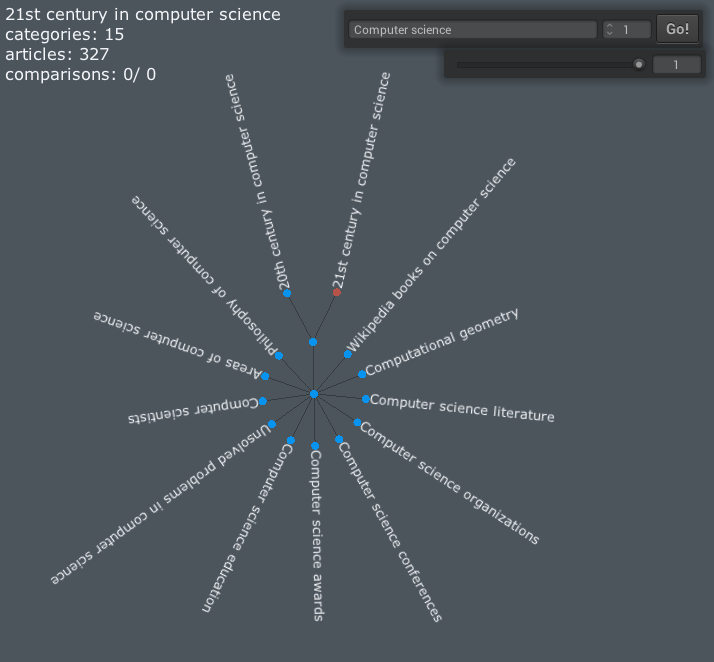
\includegraphics[scale=.21]{images/rotation-hist-1}&[3mm]&
        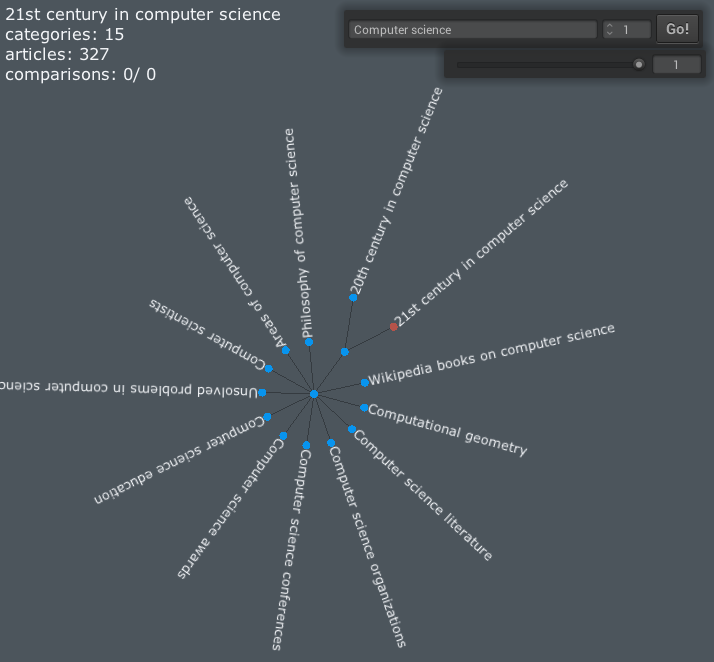
\includegraphics[scale=.21]{images/rotation-hist-2}&[3mm]&
        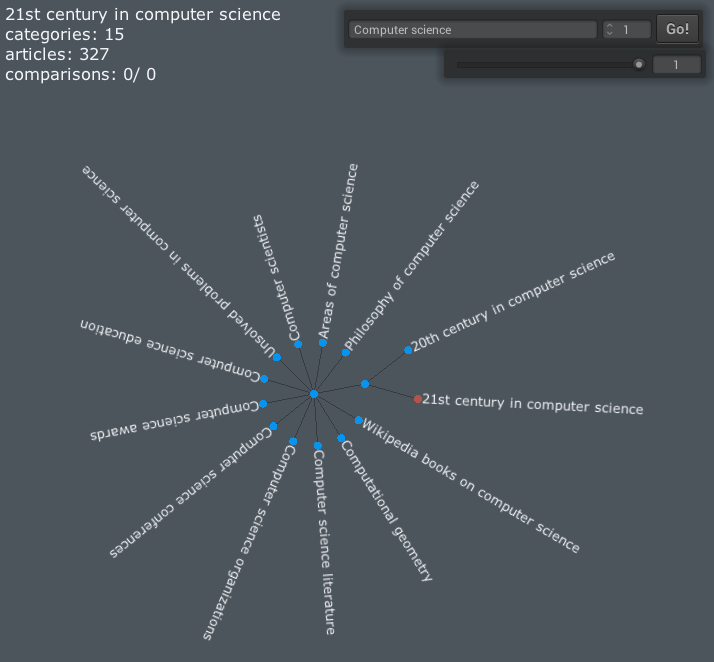
\includegraphics[scale=.21]{images/rotation-hist-3} \\
    };
    \draw[-{Latex[length=3mm]}] (m-1-1) -- (m-1-3);
    \draw[-{Latex[length=3mm]}] (m-1-3) -- (m-1-5);
    \end{tikzpicture}
    \caption{Der Kategoriebaum mit der Wurzelkategorie \emph{Computer science} und der expandierten Unterkategorie \emph{History of computer science} wird um 90\textdegree Grad im Uhrzeigersinn gedreht.}
    \label{fig:rotation-tree}
\end{figure}
% zwei bilder mit PFeil drehung der Kategorie
Die Platzierung des Mauszeigers über einer bestimmten Kategorie für dazu, das der Titel der Kategorie in der zusammenfassenden Statistik in der ersten Zeile dargestellt wird, verdeutlicht in Abbildung \ref{fig:small-start} in Bereich (b).
Auf diese Art ist es realisierbar die Titel von Kategorien anzeigen zu lassen, die keine Blattkategorien sind, ohne dabei gezeichnete Elemente zu Überlappen.

Eine essenzielle Interaktion der Visualisierung ist die Expansion von gewählten Kategorien.
Die Expansion einer Kategorie wird durch doppeltes klicken auf die Kategorie ausgeführt, dabei werden die Unterkategorien der Ausgangskategorie dem Kategorienbaum hinzugefügt und als Knoten in die Visualisierung gezeichnet.
Die neuen Unterkategorien werden durch Kanten mit der Ausgangskategorie verbunden, in Abbildung \ref{fig:expand-cat} wird dies verdeutlicht.
Die Expansion ermöglicht dabei einem Nutzer einen bestimmten Pfad von Unterkategorien zu erkunden und auf diese Weise eine differenziertere Erkundung der Unterkategorien eines Themengebietes.
Es wird neben der Expansion des Kategorienbaum für alle Blattkategorien, eine feinere Interaktion zur Verfügung gestellt.
Die Expansion, ausgehend von eine bestimmten Kategorie, ist als semantische Vertiefung zu verstehen, in der die neuen Unterkategorien eine Spezifizierung des umschriebenen Konzptes der Ausgangskategorie darstellen.
Die Expansion stellt dabei immer ein Spezifizierung der Abstraktionsebene dar, da nur Unterkategorien dem Kategorienbaum hinzugefügt werden können.

\begin{figure}
    \centering
    \begin{tikzpicture}
    \matrix (m) [matrix of nodes, nodes in empty cells] %, row 1/.style={nodes={minimum height=90mm}}]
    {
        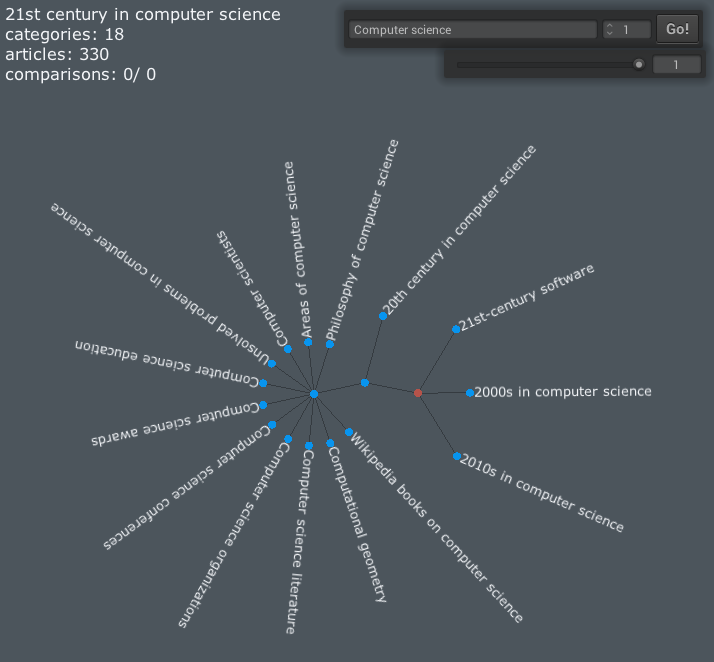
\includegraphics[scale=.3]{images/expand-hist/expand-hist-3.png}&[3mm]&
        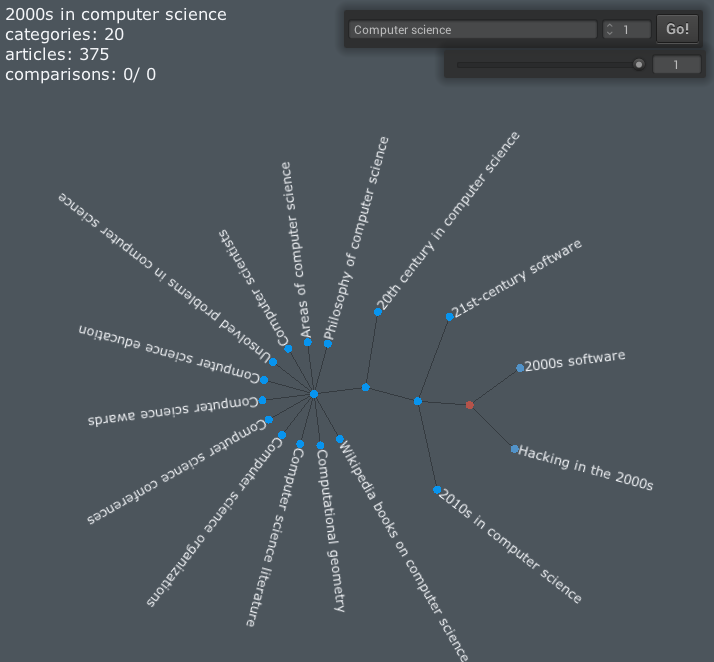
\includegraphics[scale=.3]{images/expand-hist/expand-hist-4.png}&[3mm]&\\
    
        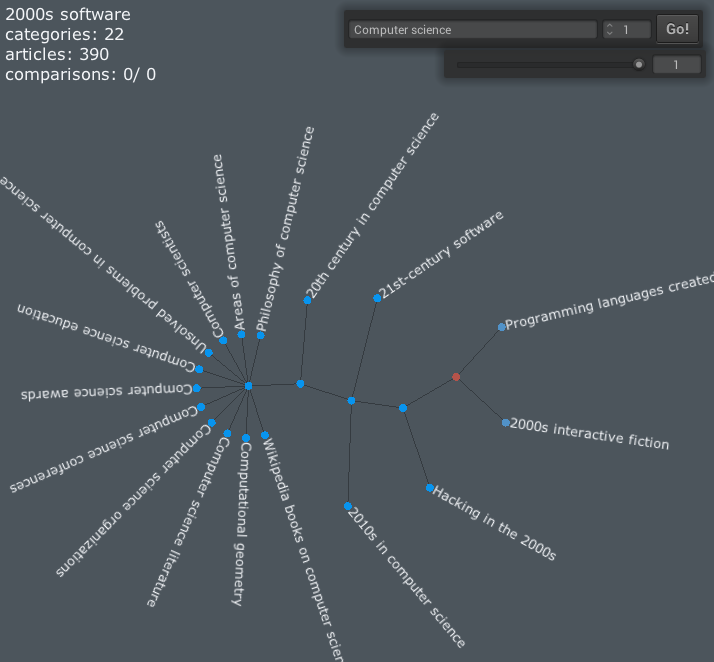
\includegraphics[scale=.3]{images/expand-hist/expand-hist-5.png}&[3mm]&
        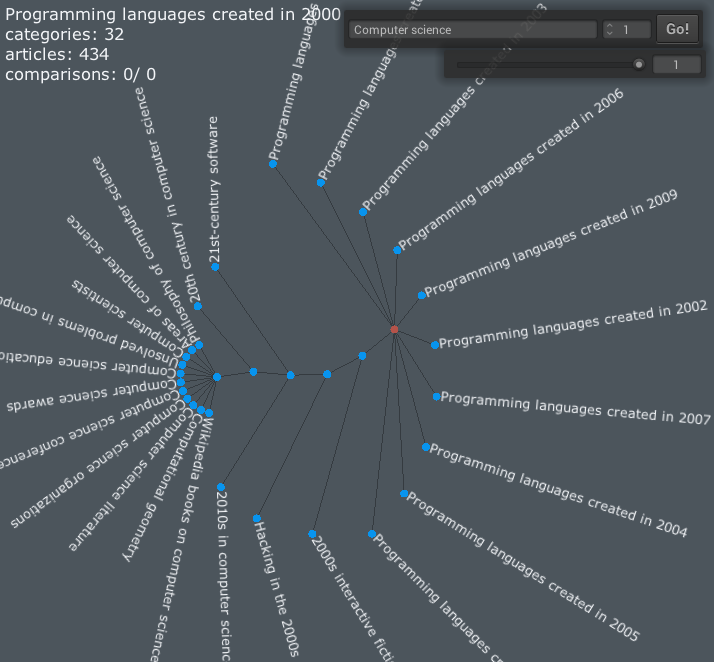
\includegraphics[scale=.3]{images/expand-hist/expand-hist-6.png}&[3mm]\\
    };
    \draw[-{Latex[length=3mm]}] (m-1-1) -- (m-1-3);
    % \draw[-{Latex[length=3mm]}] (m-1-3) -- (m-1-3);
    \draw[-{Latex[length=3mm]}] (m-2-1) -- (m-2-3);
    \end{tikzpicture}
    \caption{Die Bildabfolge stellt mehrere Expansionen vo Unterkategorien der Kategorie \emph{History of Computer science} dar. Die expandierten Kategorien sind in rot gefärbt}
\end{figure}

Mit einem einfachen Klick auf eine Kategorie, wird die Kategorie rot gefärbt um diese von andern Kategorien unterscheiden zu können.
Diese Auswahl einer Kategorie ergibt in Kombination mit der Änderung des Schwellwertes eine neue Interaktion.
Durch die Fokussierung der Kategorie werden nur Kategorien gelb gefärbt wenn sie zwei Bedingungen erfüllen.
Die Kategorien müssen Artikel eingetragen haben die eine Ähnlichkeit zur fokussierten Kategorie aufweisen und diese Ähnlichkeit muss über dem Schwellwert liegen.
In Abbildung \ref{fig:simM-threshold-focus-cat} wird noch einmal dargestellt auf welche Art diese Interaktion sich in der Ähnlichkeitsmatrix abbildet.
Die Kategorie fokussierte Variante der Schwellwertänderung, soll die Möglichkeit geben die Menge an Betrachteten Kategorien und zugehörigen Artikel weiter einschränken zu können, um eine Analyse zu vereinfachen.

\begin{figure}
    \centering
    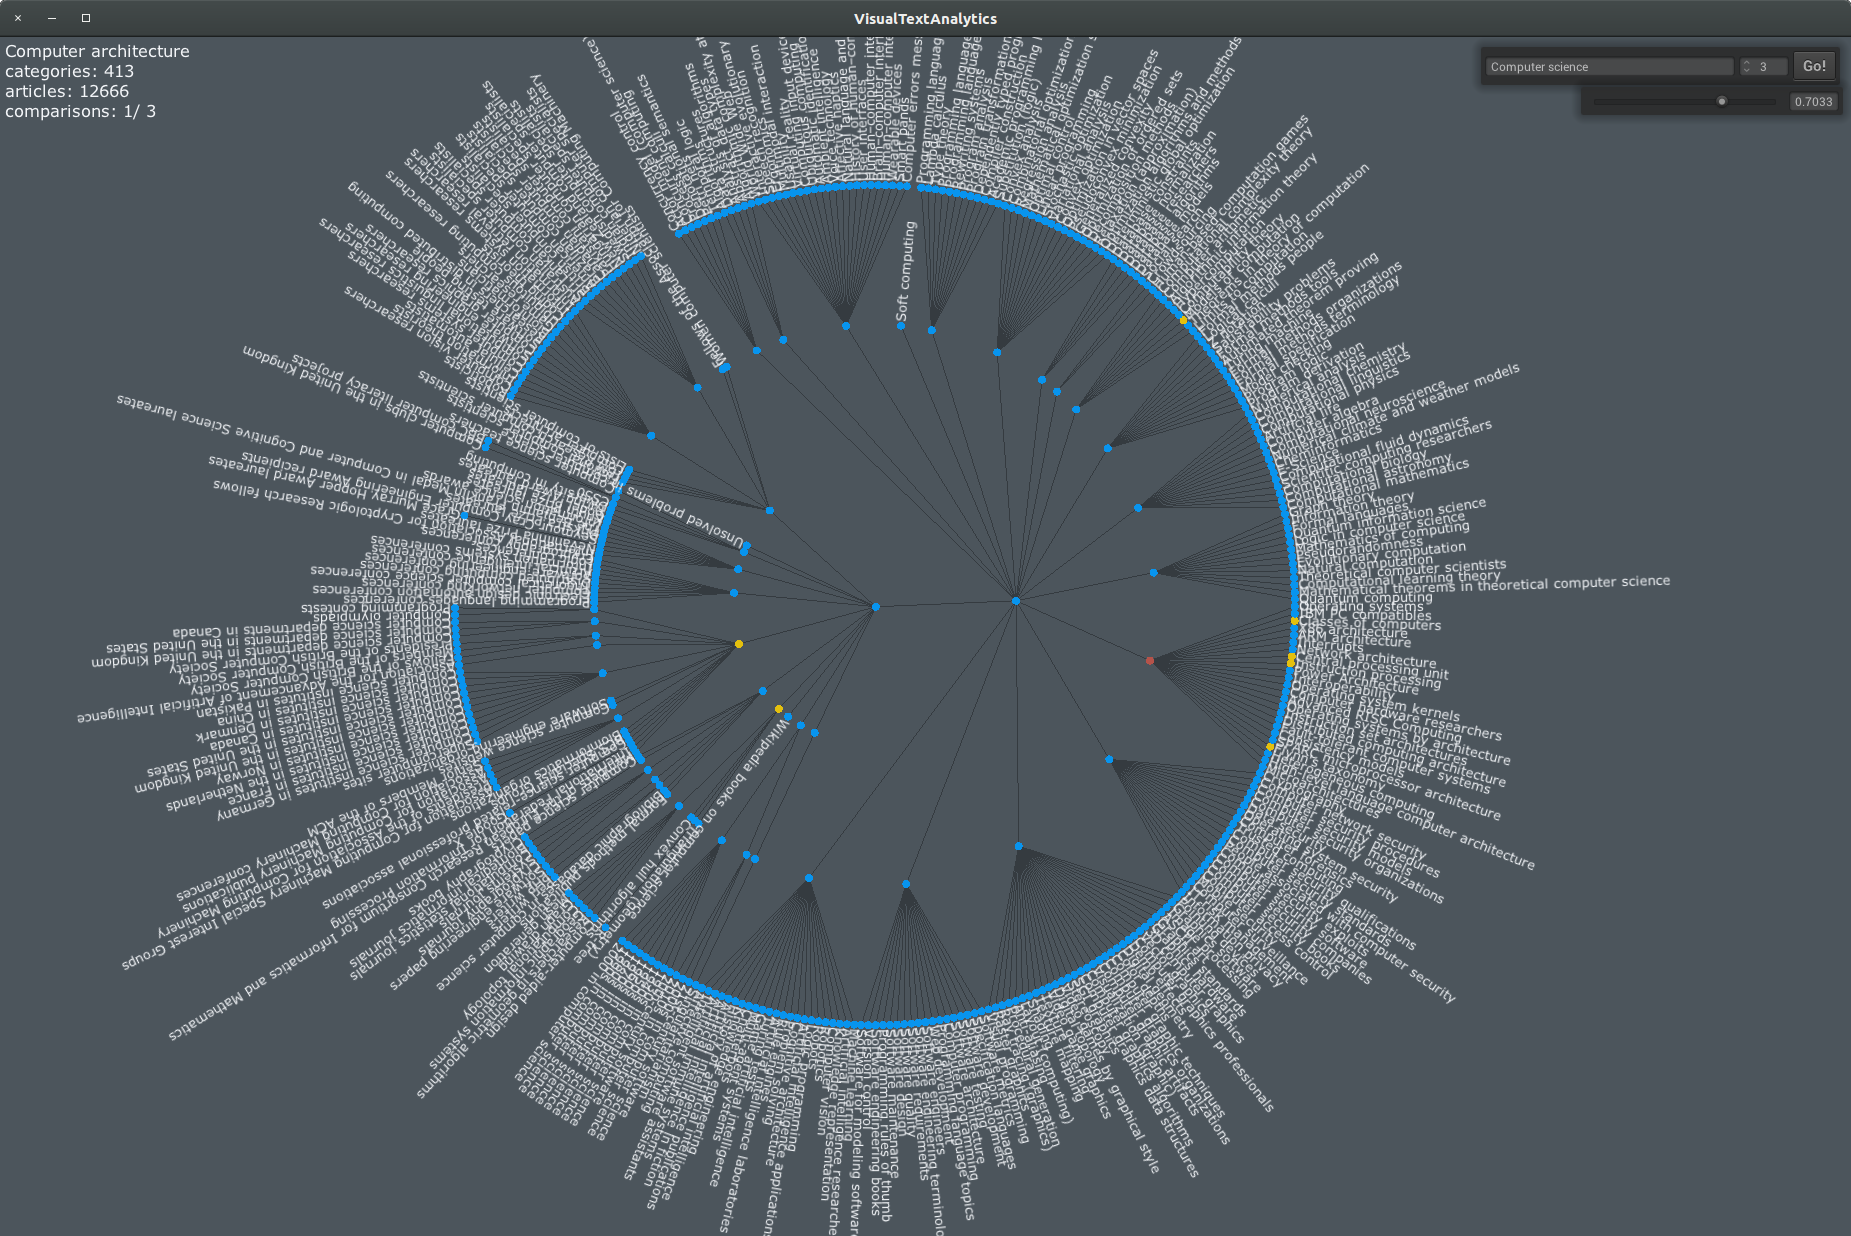
\includegraphics[width=\textwidth]{images/threshold-7033-lvl3-focus}
    \caption{Die rot gefärbte Kategorie \emph{Computer architecture} wurde fokusiert. In den gelb gefärbten Kategorien sind Artikel mit einer Ähnlichkeit zur rot gefärbten Kategorie eingetragen. Der Ähnlichkeitswert eines Artikepaares hat mindestens den Wert des Schwellwertes von $0.7033$}
    \label{fig:threshold-focus-cat}
\end{figure}

\begin{figure}
    \begin{tikzpicture}
    \end{tikzpicture}
    \caption{Darstellung der filterung der Ähnlichkeitsmatrix die durch den Schwellwert entstehen, in Kombination mit einer fokussierten Kategorie}
    \label{fig:simM-threshold-focus-cat}
\end{figure}


% Wird eine Zahl eingegeben die kleiner ist als die letztee Eingebe tiefe??

Ein Nutzer gibt in der Suchleiste den Namen einer Kategorie ein, dabei wird im Hintergrund die Datenbank mit allen Wikipediakategorien nach der Existenz der gesuchten Kategorie überprüft.
Entspricht der gesuchte Begriff nicht eine Wikipediakategorie wird der Nuzer aufgefordert einen neuen Suchbegriff einzugeben.
Die Schaltfläche "`GO"' recht von der Suchleiste Angeordnet wird rot gefärbt um darauf aufmerksam zu machen, dass die Suche erfolglos war. 
Abbildung~\ref{fig:wrong-cat} zeigt die Suchleiste mit rotgefärbter Schaltfläche.


\subsection{Benutzeroberfläche}
Abbildung \ref{fig:small-start} stellt die Benutzeroberfläche der Visualiserung dar.
Es wird der Kategorienbaum für die Stammkategorie \emph{Computer Science} und dessen direkte Unterkategorien abgebildet.
Die Benutzeroberfläche besteht dabei aus vier Elementen, dem Hauptfenster in dem der Kategorienbaum gezeichnet wird (a), einer zusammenfassenden Statistik über die Daten (b), einer Suchleiste (c) und einem Regler für den Schwellwert (d). 



\section{Laufzeit}
\section{Filterung der "Ahnlichkeitsmatrix}
% \begin{itemize}
%     \item Erl"auterung der Auswahl von Artikel aus der "Ahnlichkeitsmatrix
% \end{itemize}





%% Kapitel Visualisierung realisiesrung
Der Datensatz über die Ähnlichkeiten zwischen den Artikeln soll im Hintergrund auf diejenigen Artikel reduziert werden, welche den explorierten Kategorien entsprechen.
Auf diese Art soll die Matrix mit mehreren Billionen Vergleichen nicht nur auf eine überschaubare Menge reduziert werden, die klein genug ist, um sie schnell zu verarbeiten, sondern auch auf ein Themengebiet eingeschränkt werden.
Der Grundgedanke ist dabei, dass die Nachvollziehbarkeit von Ähnlichkeitswerten erleichtert wird, da sich die Artikel bereits thematisch ähneln und zudem eventuell ein ähnliches Vokabular benutzen.
Die Vermutung liegt nahe, dass in einem abgeschlossenen Themengebiet die Vergleichswerte zwischen den Artikeln sehr hoch sein werden.


